\section{Metadades}\label{sec:metadata-processing}

Les metadades són el conjunt d'etiquetes presents als registres d'\gls{UPCommons} que contenen informació sobre aquest.
Els autors, la descripció del recurs, la data de pujada, el departament responsable, el tipus de document, o més, es troben inclosos. \\

\noindent
En el nostre cas, a \gls{UPCommons}, aquestes utilitzen el format \gls{DSpace} Intermediate Metadata, \gls{DIM}.
Es basa a fer servir el format Dublin Core incorporant un qualificador, amb la finalitat d'afinar la informació que .
L'estructura és la següent:

\begin{center}
    \textit{schema.element.qualifier} \\
\end{center}

\noindent
Per exemple, l'autor principal d'un recurs s'identificaria com:

\begin{center}
    \text{dc.contributor.author} \\
\end{center}

\noindent
Per cada metadada, s'assignen els següents valors:

\begin{itemize}
    \item \textbf{value}: Valor de la metadada.
    \item \textbf{language}: Idioma.
    És habitual trobar-lo a les descripcions / resums dels registres, encara que a vegades no està ben introduït.
    \item \textbf{authority}: Codi que relaciona la metadada amb un sistema d'autoritats que permet obtenir més dades.
    \item \textbf{qualifier}: Un nivell de confiança associat a l'autoritat.
\end{itemize}

\clearpage

\noindent
A continuació es mostren algunes metadades extretes d'un recurs, on es pot contemplar tant el format de les metadades, com els valors. \\

\begin{tcolorbox}[colback=green!5!white, colframe=green!50!black, title=Metadades]
    Al web només hi apareix el \textbf{\textit{value}} o el \textbf{\textit{language}} de la metadada, els altres camps s'emmagatzemen internament.
\end{tcolorbox}

\begin{figure}[htbp]
    \centerline{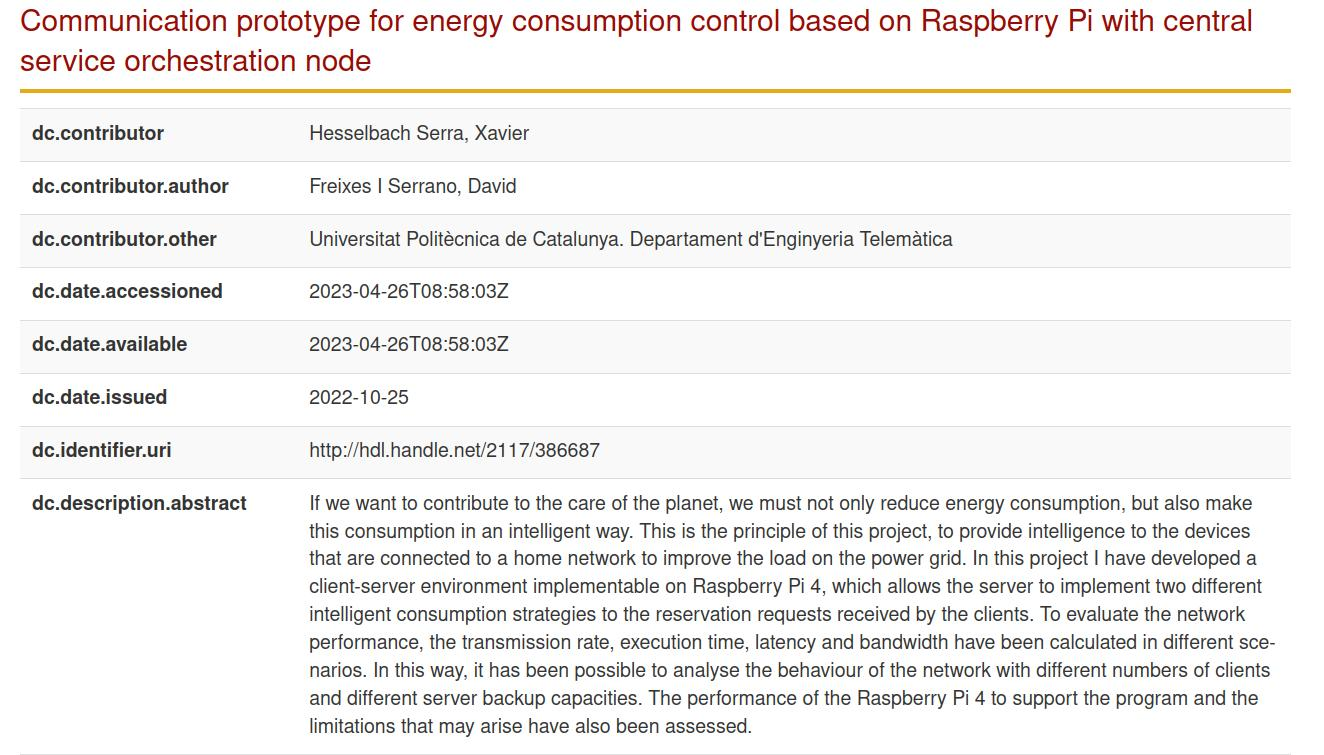
\includegraphics[width=\textwidth]{figures/metadata-example}}
    \captionsetup{justification=centering}
    \caption{Llista parcial de les metadades d'un recurs. (\textbf{Font}: \url{http://hdl.handle.net/2117/386687})}\label{fig:metadata-example}
\end{figure}

\clearpage

\subsection{\gls{OAI-PMH}}\label{subsec:oai-pmh}

El protocol \gls{OAI-PMH} (Open Archive Initiative-Protocol for Metadata Harvesting) és un estàndard d'interoperabilitat desenvolupat per l'intercanvi i la difusió de metadades. \\

\noindent
Permet accedir a metadades codificades en diferents formats, encara que el més habitual és el Dublin Core. \\

\noindent
Aquest protocol defineix sis operacions bàsiques~\cite{oai-pmh}:

\begin{itemize}
    \item \textbf{\texttt{GetRecord}}: utilitzat per obtenir informació sobre un registre individual.
    \item \texttt{\textbf{Identify}}: emprat per aconseguir informació sobre el repositori.
    \item \texttt{\textbf{ListIdentifiers}}: retorna les capçaleres dels registres.
    \item \texttt{\textbf{ListMetadataFormats}}: retorna els formats de metadades disponibles al repositori.
    \item \texttt{\textbf{ListRecords}}: verb principal per la recol·lecta de metadades, retorna els registres complets.
    \item \texttt{\textbf{ListSets}}: retorna l’estructura dels \textit{sets} del repositori.
\end{itemize}

\clearpage

\subsection{Control de Flux}\label{subsec:flux-control}

Alguns servidors implementen un mecanisme de control de flux per tal de tractar les peticions que retornin llistes incompletes.
Es basa a utilitzar un identificador anomenat \textit{resumptionToken}, que retorni la petició anterior amb la llista incompleta, i sigui paràmetre de la següent petició. \\

\begin{tcolorbox}[colback=blue!5!white, colframe=blue!75!black, title=Finestra lliscant]
    Per comparar-ho amb altres protocols, \gls{TCP}~\cite{tcp} utilitza el valor de la ``finestra lliscant'' per indicar la quantitat de dades que ha d'enviar l'emissor,
    i per \textbf{on} ha de començar, ja que aquest valor es suma al número de seqüència.
\end{tcolorbox}

\noindent \\
El procés s'iterarà fins a obtenir la llista completa.
Podrem identificar el final, pel fet que:

\begin{itemize}
    \item Aquesta darrera llista té una grandària inferior a les anteriors (acostuma a ser 100 unitats).
    \item El valor del \textit{resumptionToken} és nul. \\
\end{itemize}

\noindent
L'objectiu és, altrament que la fragmentació de peticions que demanen quantitats ciclòpiques de dades és més operatiu,
permet la recuperació del context en cas d'errors de xarxa o d'altra classe.

\clearpage

\subsection{Implementació}\label{subsec:metadata-implemntation}

L'objectiu és clar, descarregar totes les metadades.
El protocol està ben definit.
La llibreria Sickle~\cite{Sickle} ens facilita la feina.
Això resulta en una implementació senzilla:

\begin{enumerate}
    \item Connectar-se al servidor \gls{OAI} .
    \item Demanem les metadades:
    \begin{enumerate}
        \item Disposem de la llista (incompleta) de registres de metadades.
        \item Extraiem aquella informació rellevant pel nostre cas d'ús, que són les metadades en format Dublin Core.
        \item Descartem aquells registres marcats com esborrats, ja que no contenen cap informació.
        \item Realitzem l'abocament a la base de dades corresponent.
    \end{enumerate}
    \item Tornem a iterar fins a obtenir la llista completa de les metadades.
\end{enumerate}

\begin{figure}[htbp]
    \centerline{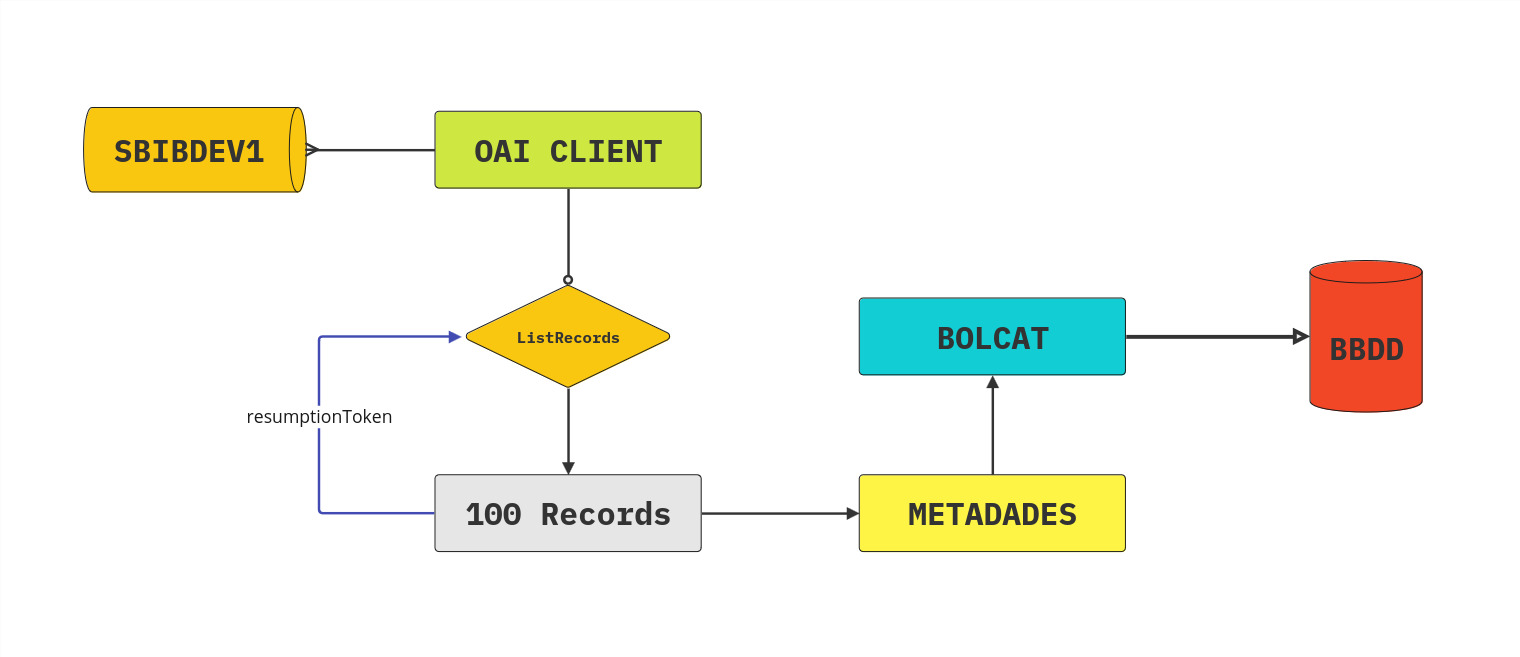
\includegraphics[width=1.2\textwidth]{figures/metadata-processing}}
    \captionsetup{justification=centering}
    \caption{Disseny tècnic del processament de les metadades. (\textbf{Font}: Elaboració pròpia.)}\label{fig:log-analysis}
\end{figure}
